\documentclass[10pt,final,leqno]{beamer}

%\usetheme{CambridgeUS}
\usetheme[style=ntnu,language=en]{ntnu2015}
%\usecolortheme{orchid}

\usepackage[utf8]{inputenc}
\usepackage[T1]{fontenc}

% Paths
\newcommand{\figs}{../figs}
\newcommand{\data}{../data}
\newcommand{\code}{../code}

% URL styles
\usepackage{url}
\urlstyle{sf}

% Units
\usepackage[detect-weight=true, binary-units=true]{siunitx}
\DeclareSIUnit\flop{FLOPS}

% Math
\usepackage{amsmath}
\usepackage{amssymb}
\usepackage{bm}
\usepackage{nicefrac}
\newcommand{\dif}[1]{{\;\text{d}#1}}

% Graphics
\usepackage{graphicx}
\usepackage{caption}
%\usepackage{subcaption}
\graphicspath{{../figs/}}

% Tikz
\usepackage{tikz}
\usetikzlibrary{positioning,shapes,arrows,calc,intersections}
\usepackage{pgfplots}
\usepgfplotslibrary{dateplot}
\pgfplotsset{compat=1.14} 

% Colors
\definecolor{darkblue}{HTML}{00688B}
\definecolor{darkgreen}{HTML}{6E8B3D}
\definecolor{cadet}{HTML}{DAE1FF}
\definecolor{salmon}{HTML}{FFB08A}

\usepackage{algorithm}

% Listings
\usepackage{textcomp}
\usepackage{listings}
\lstset{
  keywordstyle=\bfseries\color{orange},
  stringstyle=\color{darkblue!80},
  commentstyle=\color{darkblue!80},
  showstringspaces=false,
  basicstyle=\ttfamily,
  upquote=true,
}
\lstdefinestyle{fortran}{
  language=Fortran,
  morekeywords={for},
  deletekeywords={status},
}
\lstdefinestyle{c}{
  language=C,
  morekeywords={include},
}
\lstdefinestyle{glsl}{
  language=C,
  morekeywords={attribute, vec2, vec3, vec4, varying, uniform, mat2, mat3, mat4},
}
\lstdefinestyle{cuda}{
  language=C,
  morekeywords={__global__, __device__, __host__, __shared__},
}
\lstdefinestyle{shell}{
  language=bash,
  morekeywords={mkdir, ssh, cmake},
}

% Double hlines
\usepackage{hhline}

% Misc
\usepackage{nth}

\subtitle{TMA4280---Introduction to Supercomputing}

\graphicspath {{../figs/}}

\AtBeginSection[]
{
 \begin{frame}<beamer>
 \frametitle{Outline}
 \tableofcontents[currentsection]
 \end{frame}
}

\begin{document}


\title{Supercomputing}
\institute{NTNU, IMF}
\date{January 12. 2018}
\maketitle

%------------------------------------------------------------------------------
\section{Context: Challenges in Computational Science and Engineering}

\begin{frame}
  \frametitle{Computational Science and Engineering (CSE)}

\begin{center}
What is the motivation for Supercomputing?
\end{center}

\vspace{2ex}

Solve complex problems fast and accurately:
\begin{itemize}
\item efforts in modelling and simulation push sciences and engineering applications forward,
\item computational requirements drive the development of new hardware and software.
\end{itemize}

\end{frame}

%----------------------------------------
\begin{frame}
  \frametitle{Computational Science and Engineering (CSE)}

\begin{center}
Development of computational methods for scientific research\\ and innovation in engineering and technology.
\end{center}

Covers the entire spectrum of natural sciences, mathematics, informatics:
\begin{itemize}
\item Scientific model (Physics, Biology, Medical, \dots)
\item Mathematical model
\item Numerical model
\item Implementation
\item Visualization, Post-processing
\item Validation
\end{itemize}
$\rightarrow$ Feedback: virtuous circle

\begin{center}
Allows for larger and more realistic problems to be simulated, new theories to be experimented numerically.
\end{center}

\end{frame}

%----------------------------------------
\begin{frame}
  \frametitle{Outcome in Industrial Applications}

\begin{figure}
\centering
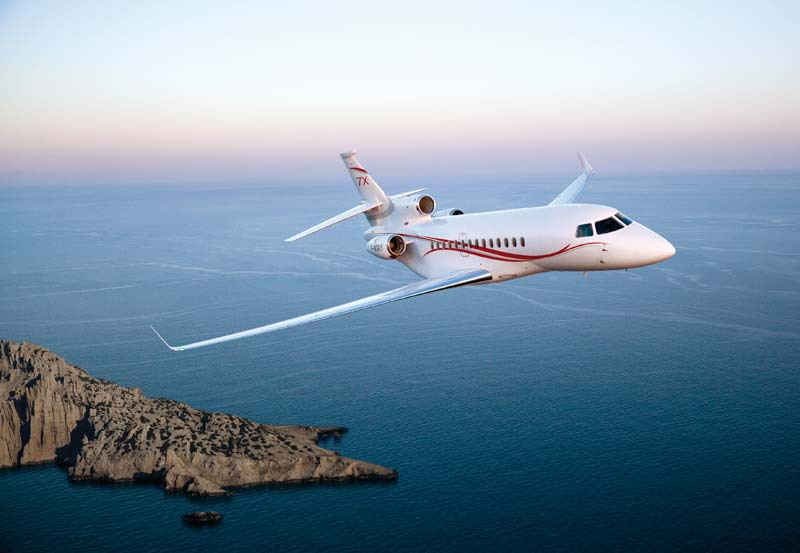
\includegraphics[width=0.7\linewidth]{dassault/Falcon7X}
\caption{2004: ``The Falcon 7X becomes the first aircraft in industry history to be entirely developed in a virtual environment, from design to manufacturing to maintenance.'' Dassault Systèmes}
\end{figure}

\end{frame}

%----------------------------------------
\begin{frame}
  \frametitle{Evolution of computational power}
\begin{figure}
\centering
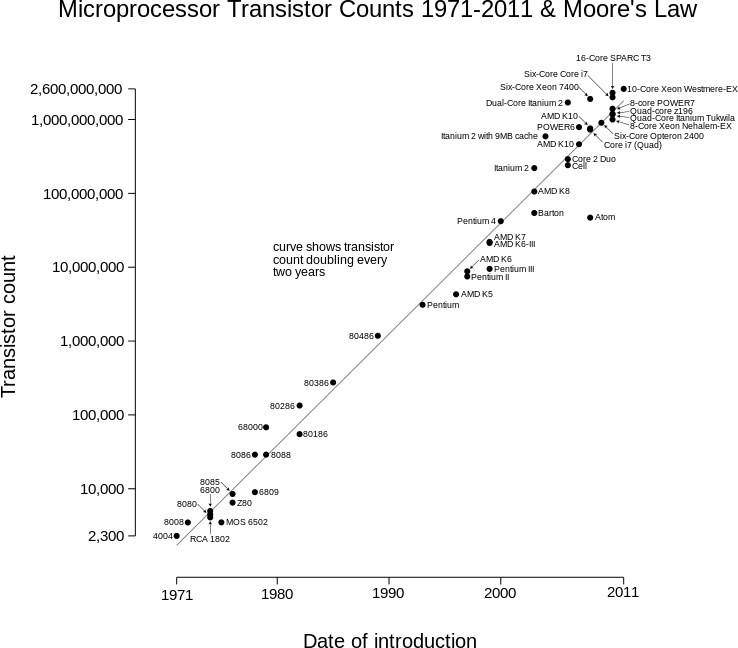
\includegraphics[width=0.7\linewidth]{wikimedia/MooreLaw}
\caption{Moore's Law: exponential increase of number of transistors per chip,  1-year rate (1965), 2-year rate (1975). WikiMedia, CC-BY-SA-3.0}
\end{figure}

\end{frame}

%----------------------------------------
\begin{frame}
  \frametitle{Evolution of computational power}


\begin{figure}
\centering
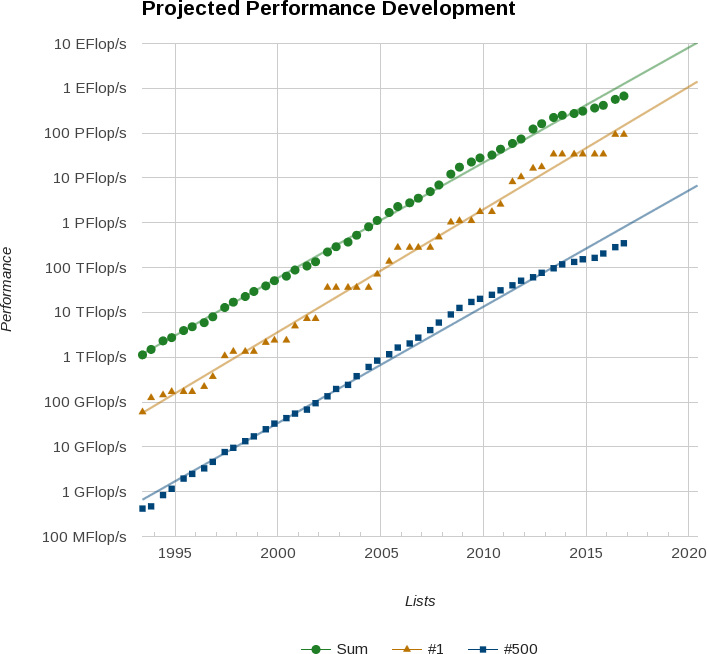
\includegraphics[width=0.7\linewidth]{top500/flops/PerformanceDevelopment}
\caption{Top500: worlwide ranking of supercomputers. Source: top500.org}
\end{figure}

\end{frame}

%----------------------------------------
\begin{frame}
  \frametitle{Progress in numerical methods and software}

Progress cannot be achieved only by raw performance:
\begin{itemize}
\item improvement of linear solvers,
\item model reduction,
\item uncertainty quantification,
\item development of new programming models,
\item \dots
\end{itemize}

Each stage of the development of a new method requires care:
\begin{itemize}
\item Implementation: unit testing
\item Algorithms: verification
\item Conceptual model: validation
\item Error propagation, Reliability: uncertainty quantification
\end{itemize}

\end{frame}

\section{Examples: Simulation of turbulent flows and other applications}

\begin{frame}
  \frametitle{Context}

Why is it necessary to
\begin{itemize}
\item solve larger problems,
\item improve accuracy,
\end{itemize}
and how to work towards these goals?

\end{frame}

%----------------------------------------
\begin{frame}
  \frametitle{Example: Large-Eddy Simulation}

\newcommand{\uu}{{\boldsymbol u}}
\newcommand{\ff}{{\boldsymbol f}}
\newcommand{\Div}{{\boldsymbol\nabla\cdot}}
\newcommand{\Grad}{{\boldsymbol\nabla}}

\textbf{Incompressible Navier--Stokes Equations (NSE):}\\
\begin{equation*}\label{icnseq}
      \left\lvert
      \begin{array}{rcll}
      \mbox{Find $\hat \uu\equiv (\uu, p)$ such that:}\\[2ex]
	    \partial_t  \uu+(\uu\cdot\Grad)\uu+ \Grad p - 2\nu \Div\;\varepsilon(\uu) &=& \ff 
      
      \,\, &\mbox{in } \Omega\times[0,T]\\ 
      \Div \uu&=& 0\,\, &\mbox{in }\Omega\times[0,T]\\
       \hat \uu(\cdot ,0) &=&  \hat \uu^0\,\, &\mbox{in }  \Omega
      \end{array}
      \right.
\end{equation*}

\begin{itemize}
\item Scope: 3D turbulent flows, high Reynolds number $Re = 10^5-10^6$
\item Applications: design of turbines, aircrafts, climate modelling, \dots
\item Discretization: finite dimensional problem, $N$ degrees of freedom,
\item Modelling unresolved scales: physical subgrid model, stabilization (Implicit LES), filtering \dots
\end{itemize}

Number of degrees of freedom to resolve scales, Kolmogorov Law:
\begin{equation*}
N \sim Re^{9/4}
\end{equation*}

\end{frame}

%----------------------------------------
\begin{frame}
  \frametitle{AIAA Benchmark: Complex Landing Gear (BANC-II)}

\begin{itemize}
\item Meshes: initial 3.6M elements, final 23.8M elements
\item Resources: adaptive stages 900K core.h, final 600K core.h
\end{itemize}
\begin{figure}[hbt]
  \centering
  \href{run:\figs/ctl/banc2.mp4}{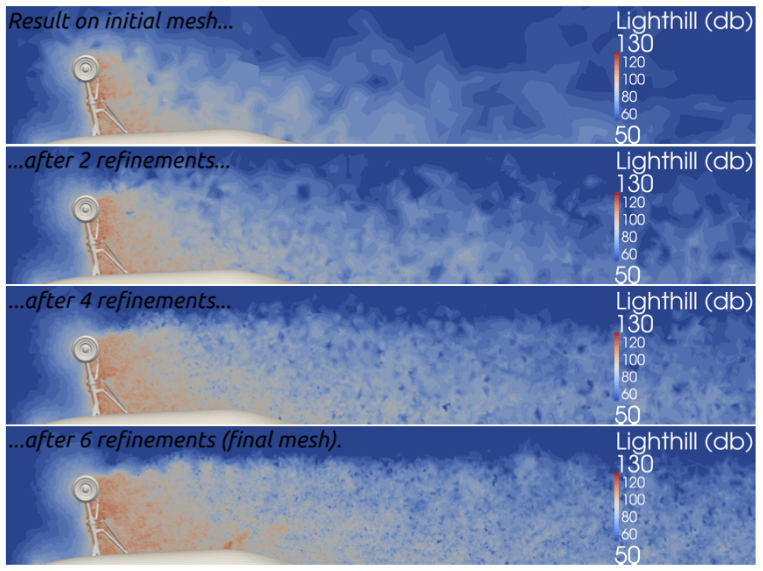
\includegraphics[width=0.7\linewidth]{ctl/banc2_stages}}
  \caption{Mesh adaptation stages, Lighthill tensor (noise generation). Vilela De Abreu/N. Jansson/Hoffman, 18th AIAA Aeroacoustics Conference, 2012}
\end{figure}

\end{frame}

%----------------------------------------
\begin{frame}
  \frametitle{Applications}

Computationally intensive problems:
\begin{itemize}
\item Physical phenomena involving a large range of scales
\item Systems with many degrees of freedom
\item Methods with high dimensionality (Monte--Carlo)
\item Big Data 
\end{itemize}

\end{frame}

%----------------------------------------
\begin{frame}
  \frametitle{Example: weather forecasting}
  \begin{center}
    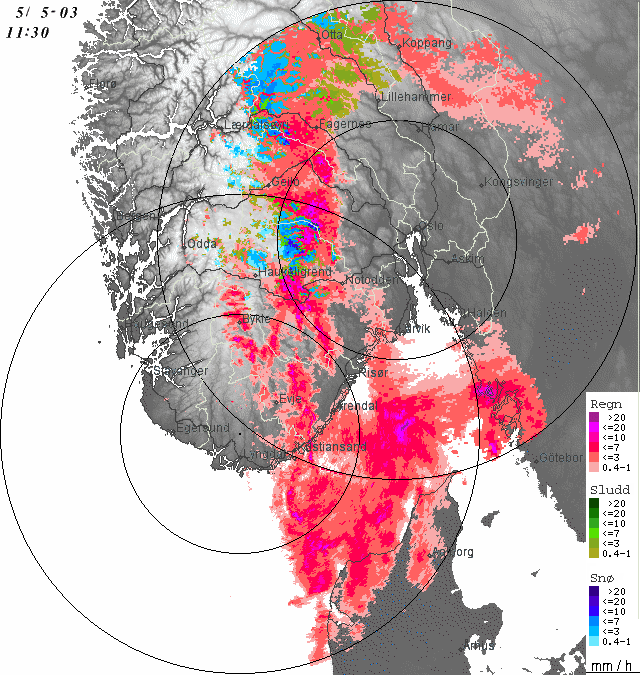
\includegraphics[height=0.7\textheight]{met} \\
    For more information, see \url{http://met.no}
  \end{center}
\end{frame}

%----------------------------------------
\begin{frame}
  \frametitle{Example: climate modelling}

  \begin{center}
    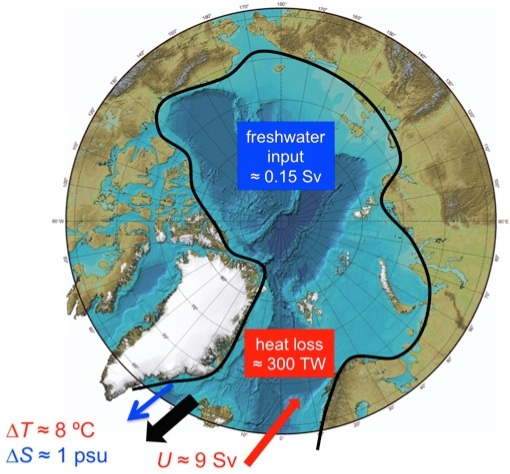
\includegraphics[height=0.7\textheight]{climate_model} \\
    For more information, see \url{http://www.bjerknes.uib.no}. \\
    Source: Nilsen et al. (2008)
  \end{center}
\end{frame}

%----------------------------------------
\begin{frame}
  \frametitle{Example: molecular dynamics}
  \begin{center}
    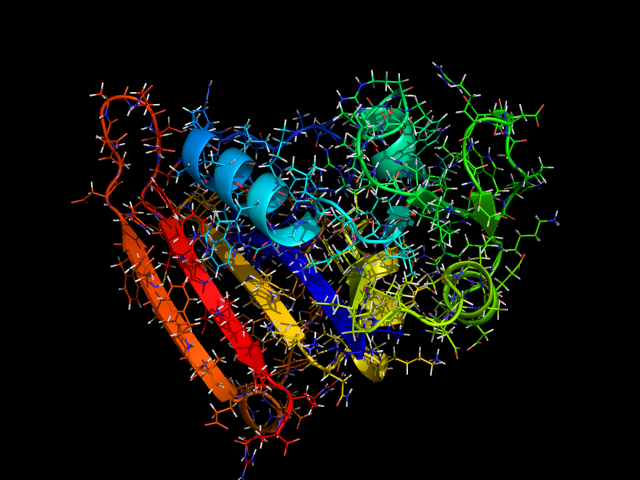
\includegraphics[width=0.8\textwidth]{gromacs/dhfr_implicit} \\
    For more information, see \url{http://www.gromacs.org}.
  \end{center}
\end{frame}

%------------------------------------------------------------------------------
\section{Goal and means: parallel performance improvement}

%----------------------------------------
\begin{frame}
  \frametitle{Evaluation of performance}

Measure unit: \SI{}{\flop}, Floating-point Operator Per Second.

\vspace{2ex}

\begin{enumerate}
\item $R_{PEAK}$: theoretical operation rate handled by the hardware.
\item $R_{MAX}$: maximum achieved in reality for a given benchmark.
\end{enumerate}

\begin{center}
Efficiency: $\mathcal{E} = R_{MAX} / R_{PEAK}$
\end{center}

Top500: ranking using HPL (High-Performance LINPACK Benchmark)
LINPACK: library for solving dense linear systems.

\end{frame}

%----------------------------------------
\begin{frame}
  \frametitle{Parallelization}

Example of mesh distribution:
\begin{center}
   \begin{minipage}[bc]{0.48\linewidth}
   \centering
   \begin{figure}
    \centering
    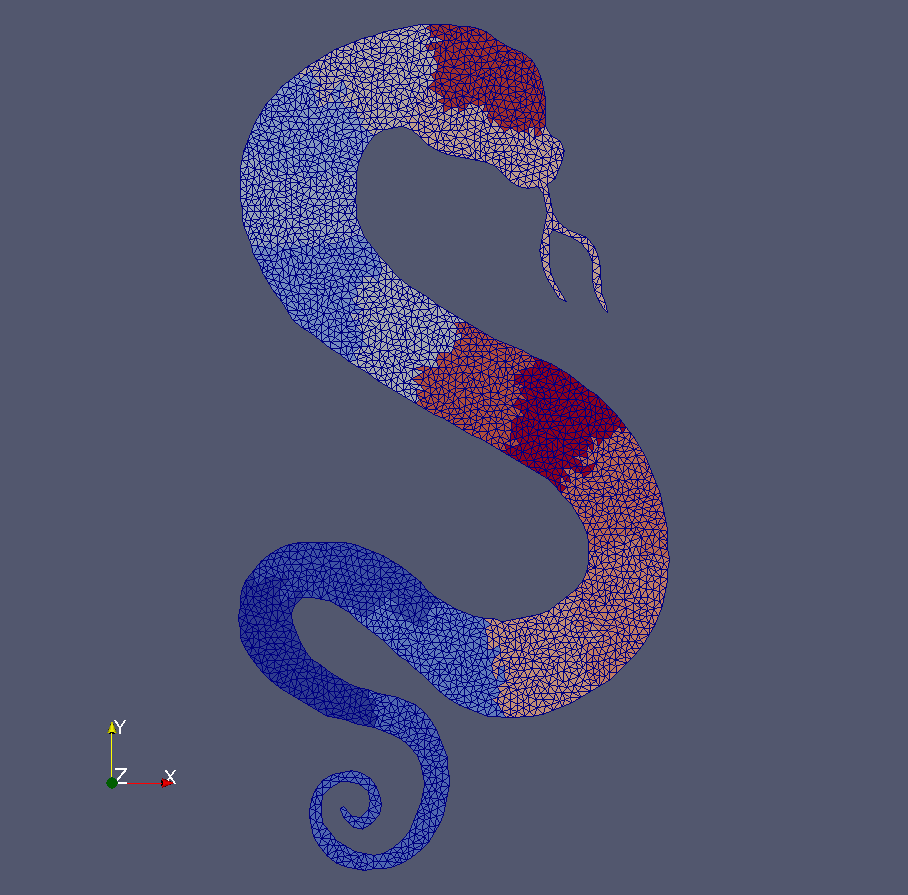
\includegraphics[width=\linewidth]{dolfin/snake}
    \caption{\label{fig:snake} Snake demo run, 16 processes.}
\end{figure}
   \end{minipage}
   \hfill
   \begin{minipage}[bc]{0.48\linewidth}
   \centering
   \begin{figure}
    \centering
    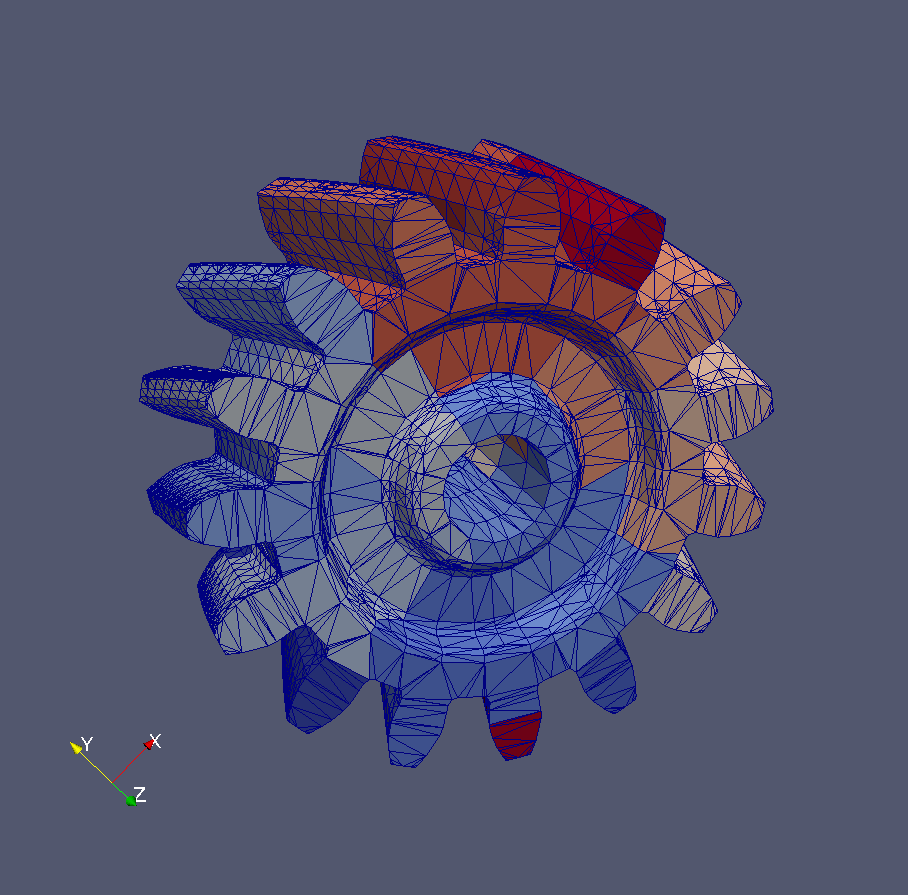
\includegraphics[width=\linewidth]{dolfin/gear}
    \caption{\label{fig:gear} Gear demo run, 32 processes.}
    \end{figure}
   \end{minipage}
\end{center}

\end{frame}

%----------------------------------------
\begin{frame}
  \frametitle{Expectations and limitations}

\begin{itemize}
\item Given a fixed problem:
\begin{center}
Serial computation $\rightarrow$ Parallel computation on P processors
\end{center}

\vspace{2ex}
\item The \textbf{wall time} $T_n$ is the execution time on $n$ processors. 

\vspace{2ex}
\item Speed-up:
\begin{equation*}
S_P = T_1 / T_P
\end{equation*}

\vspace{2ex}

\item Ideally, linear (strong) scaling: $S_P = P$

\vspace{2ex}

\item Data dependencies, Communication overhead, \dots
\end{itemize}

\end{frame}

%----------------------------------------
\begin{frame}
  \frametitle{Levels of parallelism: Single processor}

Core
\begin{itemize}
\item pipelining
\item superscalar execution
\item vector processing (SIMD unit)
\item branch prediction
\item caching techniques
\item multithreading
\item prefetching
\item \dots
\end{itemize}
\begin{center}
Instruction-level parallelism, Concurrency
\end{center}

\end{frame}

%----------------------------------------
\begin{frame}
  \frametitle{Levels of parallelism: Multi-processor}

Compute node
\begin{itemize}
\item multiple cores on a chip
\item core sharing cache memory
\item affinity, locality
\item accelerators
\item \dots
\end{itemize}
\begin{center}
Shared memory model
\end{center}

\end{frame}

%----------------------------------------
\begin{frame}
  \frametitle{Levels of parallelism: Distributed system}


Cluster (system comprised of several compute nodes)
\begin{itemize}
\item network topologies
\item optimized libraries
\item communication patterns
\item \dots
\end{itemize}
\begin{center}
Distributed memory model
\end{center}

\end{frame}

%------------------------------------------------------------------------------
\section{Overview of supercomputing systems}

\begin{frame}
  \frametitle{Historical perspective: CRAY-1}
\begin{center}
\textit{``The world’s fastest from 1976 to 1982 !''}
\end{center}
\begin{minipage}[bc]{0.4\linewidth}
\begin{figure}
\centering
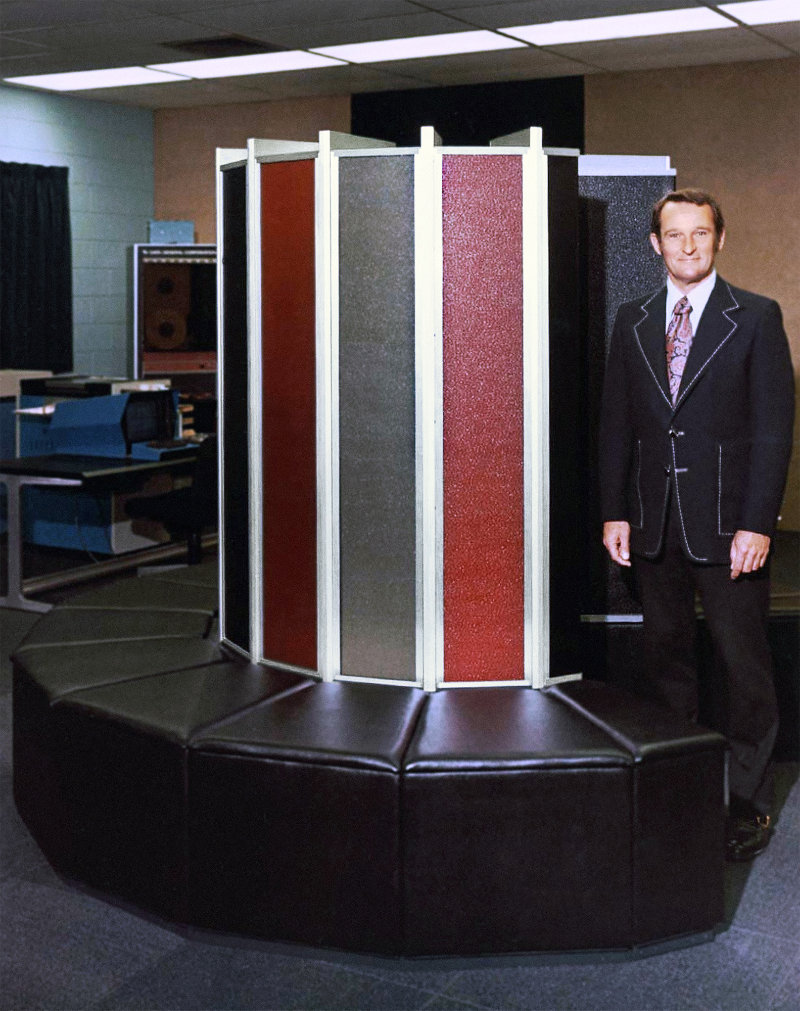
\includegraphics[width=0.8\linewidth]{computerhistory/CRAY1}
\caption{Pr. Seymour Cray and a CRAY-1. © Cray Research, Inc. (CRI)}
\end{figure}
\end{minipage}
\begin{minipage}[bc]{0.55\linewidth}
Specifications:
\begin{itemize}
\item Type: Vector computer
\item Processor Clock 83 MHz
\item Peak performance \SI{166}{\mega\flop}
\item Memory 8 MB to 32 MB
\item Sold for $\SI{8.8}{M}$ dollars
\item Power consumption of $\SI{115}{kW}$
\end{itemize}
Comparison:
\begin{itemize}
\item Intel Xeon E5-2620v3 (6 cores):\\
\SI{200}{\giga\flop}
\item Nvidia Tesla:\\
\SI{500}{\giga\flop} to \SI{1}{\tera\flop}
\end{itemize}
\end{minipage}

\end{frame}

\begin{frame}
  \frametitle{Historical perspective: evolution}

\begin{center}
Top Computers Over Time for the Highly-Parallel Linpack Benchmark.

\vspace{2em}
\scalebox{0.9}{
\begin{tabular}{|l|l|l|l|}
\hline
Year    &    Computer                                & Processors &       $R_{MAX}$ \\
\hline
2005    &    IBM Blue Gene/L                        &  131072             & 280600           \\
2002    &    Earth Simulator Computer, NEC          &  5104               & 35610           \\
2001    &    ASCI White-Pacific, IBM SP Power3      &  7424               & 7226           \\
2000    &    ASCI White-Pacific, IBM SP Power3      &  7424               & 4938            \\
1999    &    ASCI Red Intel Pentium II Xeon         &  9632               & 2379            \\
1998    &    ASCI Blue-Pacific SST, IBM SP604E      &  5808               & 2144           \\
1997    &    Intel ASCI Option Red 200MHzPentiumPro &  9152               & 1338            \\
1996    &    Hitachi CP-PACS                        &  2048               & 368.2           \\
1995    &    Intel Paragon XP/S MP                  &  6768               & 281.1        \\
1994    &    Intel Paragon XP/S MP                  &  6768               & 281.1          \\
1993    &    Fujitsu NWT                            &  140                & 124.5       \\
1992    &    NEC SX-3/44                            &  4                  & 20.0            \\
1991    &    Fujitsu VP2600/10                      &  1                  & 4.0        \\
\hline   
\end{tabular}

}
\end{center}


Achieved performance $R_{MAX}$ in GFlops.
\end{frame}

\begin{frame}
  \frametitle{Historical perspective: current consumer hardware}


\textbf{Can you estimate the computing power of a Raspberry Pi Model-B?}
\end{frame}


\begin{frame}
  \frametitle{Historical perspective: current consumer hardware}


\textbf{Can you estimate the computing power of a Raspberry Pi Model-B?}
\begin{center}

\vspace{2em}
LINPACK single node compute benchmark result:

\vspace{2em}
\begin{tabular}{|l|l|}
\hline
Precision &  $R_{MAX}$  \\
\hline
Single    &  0.065 GFLOPS  \\
Double    &  0.041 GFLOPS  \\
\hline
\end{tabular}
\end{center}

\vspace{2em}
A cluster of 64 Raspberry Pi Model B computers, labeled "Iridis-pi", achieved a LINPACK HPL suite result of:
\begin{center}
\textbf{1.14 GFLOPS} (n=10240) at \textbf{216 Watts} for power consumption.
\end{center}
\end{frame}

%The LINPACK single node compute benchmark results in a mean single precision performance of 0.065 GFLOPS and a mean double precision performance of 0.041 GFLOPS for one Raspberry Pi Model-B board.[16] A cluster of 64 Raspberry Pi Model B computers, labeled "Iridis-pi", achieved a LINPACK HPL suite result of 1.14 GFLOPS (n=10240) at 216 watts for c. US$4000.[16]

%----------------------------------------
\begin{frame}
  \frametitle{Supercomputers at NTNU: History}

Supercomputing center established in 1983.
  \begin{center}
    \scalebox{0.8}{
      \bgroup\def\arraystretch{1.2}
\begin{tabular}{llrlr}
  \hline
  Year & System & Processors & Type & $\SI{}{\giga\flop}$ \\
  \hhline{=====}
  1986--1992 & Cray X-MP & 2 & Vector & 0.5 \\
  1992--1996 & Cray Y-MP & 4 & Vector & 1.3\\
  1995--2003 & Cray J90     & 8 & Vector & 1.6 \\
  1992--1999 & Intel Paragon & 56 & MPP & 5.0\\
  1996--2003 & Cray T3E & 96 & MPP & 58\\
  2000--2001 & SGI O2 & 160 & ccNUMA & 100\\
  2001--2008 & SGI O3 & 898 & ccNUMA & 1000\\
  2006--2011 & IBM P5+ & 2976 & Distributed SMP & 23500\\
  2012--     & SGI Altix ICE X & 23040 & Distributed SMP & 497230 \\
  \hline
\end{tabular}
\egroup

    }
  \end{center}
\end{frame}

%----------------------------------------
\begin{frame}
  \frametitle{Supercomputers at NTNU: Current}
  
\begin{minipage}[bc]{0.4\linewidth}
\centering
\texttt{vilje.hpc.ntnu.no}
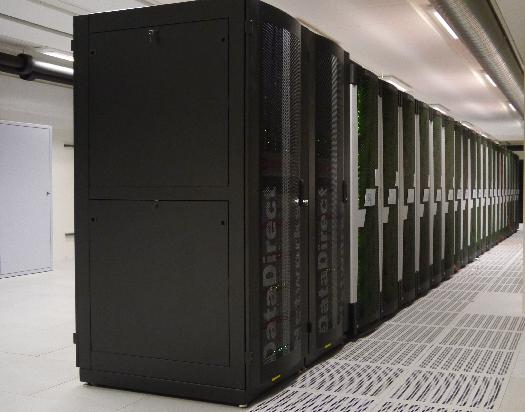
\includegraphics[width=0.8\linewidth]{sigma/vilje}
\end{minipage}
\begin{minipage}[bc]{0.55\linewidth}
\begin{itemize}
  \item System: SGI Altix ICE
  \item Type: Distributed SMP
  \item Nodes: 1404
  \item Each node is a shared memory system with two octa-core chips and
    $\SI{32}{\giga\byte}$ memory.
  \item Physical cores: 22464
  \item Logical cores: 44928
  \item CPU: Intel Xeon (Sandy Bridge)
  \item Theoretical peak performance: $\SI{467}{\tera\flop}$
  \end{itemize}
\end{minipage}

UNINETT Sigma2 manages the supercomputing infrastructure in Norway:
https://www.sigma2.no/

\end{frame}

%----------------------------------------
\begin{frame}
  \frametitle{Supercomputers at NTNU: IDUN/Lille}

\begin{minipage}[bc]{0.55\linewidth}
\begin{itemize}
  \item System: Dell P630
  \item Type: Distributed SMP
  \item Nodes: 27
  \item Each node is a shared memory system with two deca-core chips and
    $\SI{128}{\giga\byte}$ memory.
  \item CPU: Intel Xeon E5-2630v4 (about 500GFLops per CPU)
  \end{itemize}
\end{minipage}

\end{frame}


\begin{frame}
  \frametitle{Supercomputers at NTNU: IDUN/Lille}

\begin{center}
    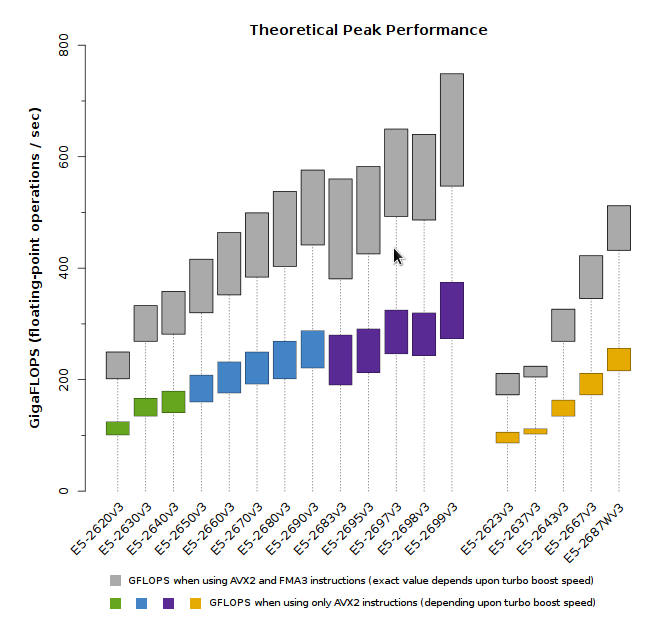
\includegraphics[height=0.7\textheight]{\figs/tma4280/broadwell}
  \end{center}

\end{frame}

%----------------------------------------
\begin{frame}
  \frametitle{Types of system architecture}

Various existing categories:
\begin{itemize}
\item vector computers (CRAY X-MP)
\item shared memory systems (SGI O3)
\item distributed memory clusters (SGI Altix ICE X)
\item compute grids (Folding@HOME)
\end{itemize}

\vspace{2ex}

Each of them require:
\begin{itemize}
\item adapting algorithms,
\item using different programming models,
\item hardware-specific implementation optimizations,
\item \dots
\end{itemize}

\end{frame}

%----------------------------------------
\begin{frame}
  \frametitle{Evolution: system architecture}

\begin{minipage}[bc]{0.4\linewidth}
\centering
\begin{figure}
\centering
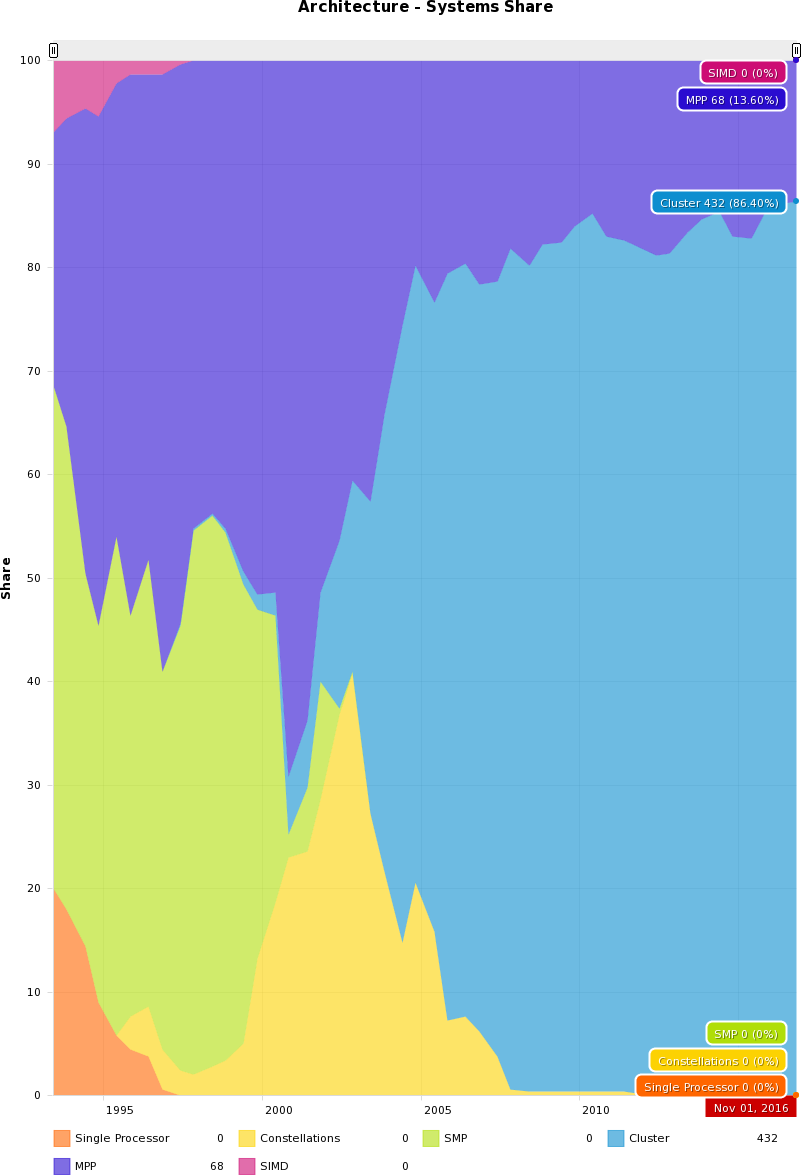
\includegraphics[width=\linewidth]{top500/architecture/Architecture_System}
\end{figure}
\end{minipage}
\begin{minipage}[bc]{0.4\linewidth}
\centering
\begin{figure}
\centering
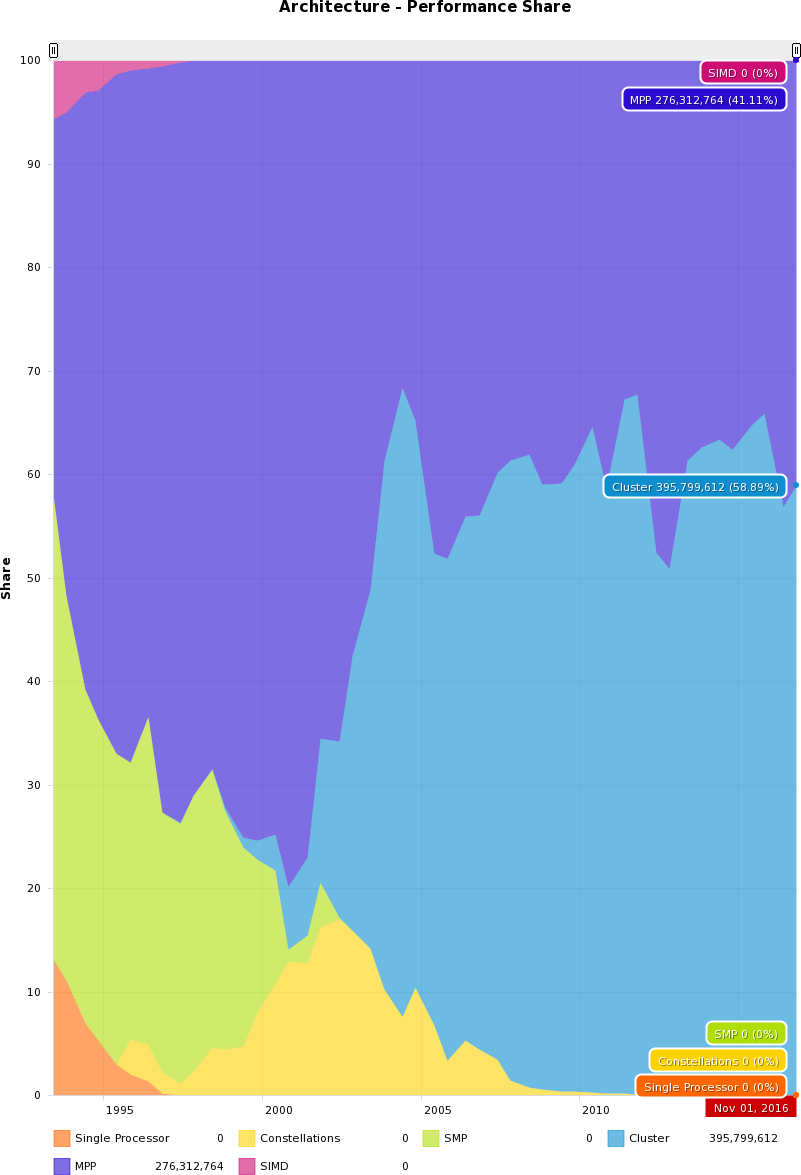
\includegraphics[width=\linewidth]{top500/architecture/Architecture_Performance}
\end{figure}
\end{minipage}

\smallskip
Comparison of the evolution w.r.t system and performance share.
\end{frame}

%----------------------------------------
\begin{frame}
  \frametitle{Back to Moore's Law}
\begin{figure}
\centering
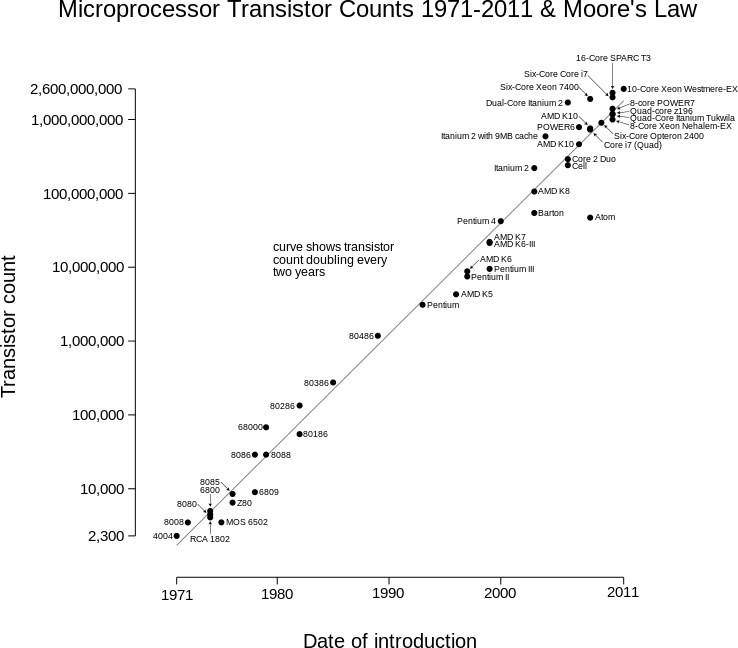
\includegraphics[width=0.7\linewidth]{wikimedia/MooreLaw}
\end{figure}

Limitations to improving single-core performance $\rightarrow$ multi-core.

\end{frame}

%----------------------------------------
\begin{frame}
  \frametitle{Evolution: number of cores per socket}

\begin{minipage}[bc]{0.4\linewidth}
\centering
\begin{figure}
\centering
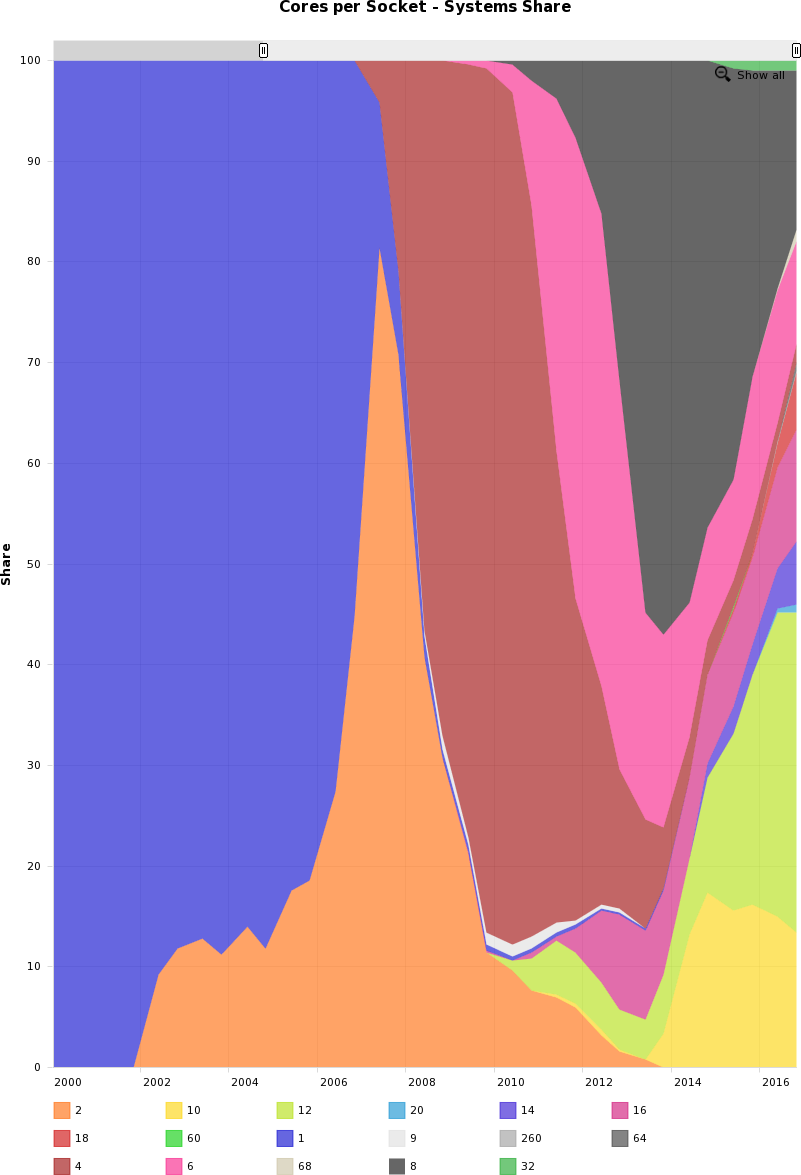
\includegraphics[width=\linewidth]{top500/cores/CoresPerSocket_System}
\end{figure}
\end{minipage}
\begin{minipage}[bc]{0.4\linewidth}
\centering
\begin{figure}
\centering
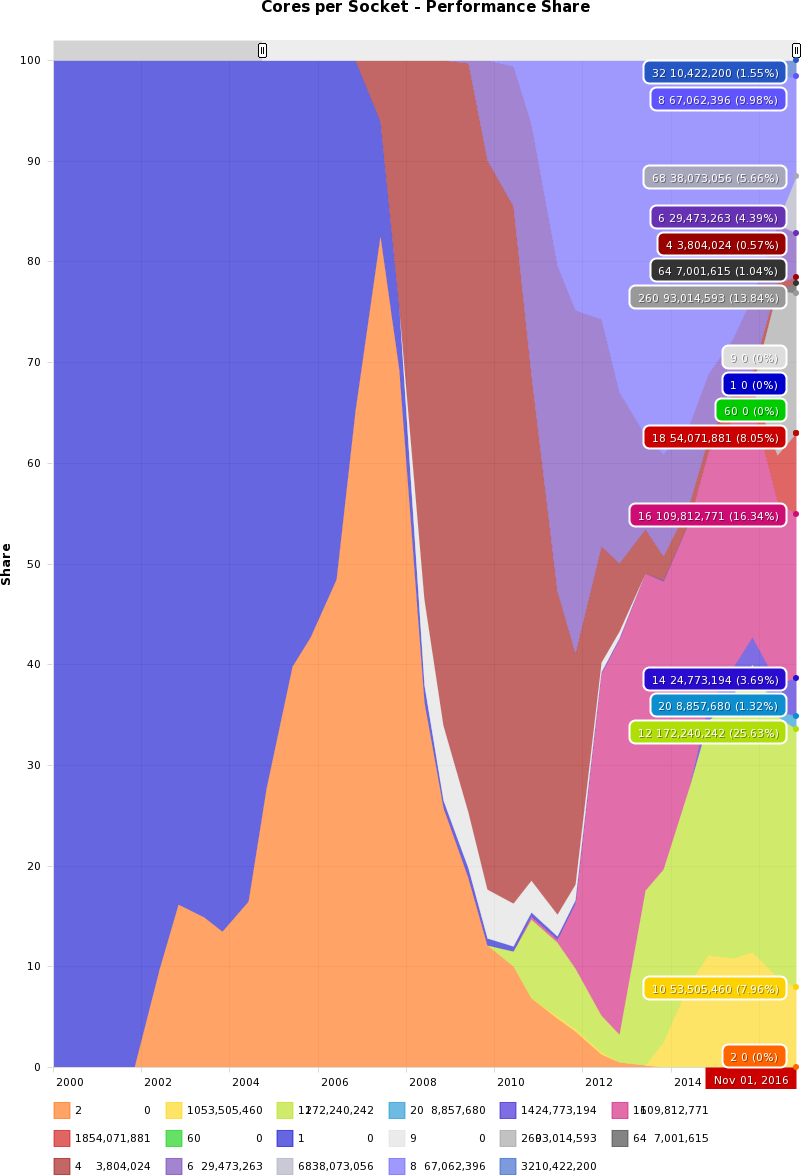
\includegraphics[width=\linewidth]{top500/cores/CoresPerSocket_Performance}
\end{figure}
\end{minipage}

\smallskip
Comparison of the evolution w.r.t system and performance share.
\end{frame}

%----------------------------------------
\frame{

\frametitle{Network}

\begin{center}
   \begin{minipage}[bc]{0.45\linewidth}
   \centering
   \begin{figure}
    \centering
    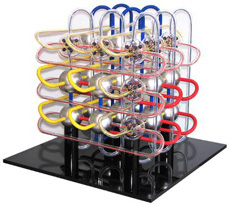
\includegraphics[width=\linewidth]{fujitsu/TOFU}
    \caption{K-Computer, 6D mesh/torus TOFU network topology, Fujitsu.}
    \end{figure}
   \end{minipage}
   \hfill
   \begin{minipage}[bc]{0.54\linewidth}
   \centering
   \vspace{8ex}
   \begin{figure}
    \centering
    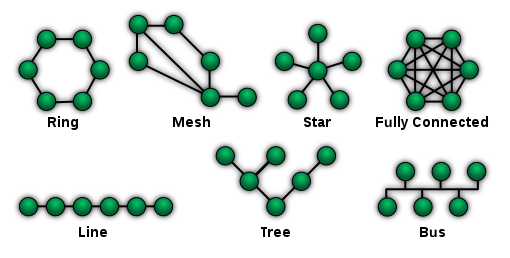
\includegraphics[width=\linewidth]{wikimedia/NetworkTopologies}
    \caption{Network topologies, WikiMedia, Public Domain}
\end{figure}
   \end{minipage}
\end{center}
Factors influencing the performance of communications:
\begin{itemize}
\item nature of the wiring (copper cable, optical fibre)
\item topology of the network to reduce the transmission path
\item protocols, algorithms  (packet ordering, error checking) 
\end{itemize}

}

%----------------------------------------
\begin{frame}
  \frametitle{Evolution: interconnect}

\begin{minipage}[bc]{0.4\linewidth}
\centering
\begin{figure}
\centering
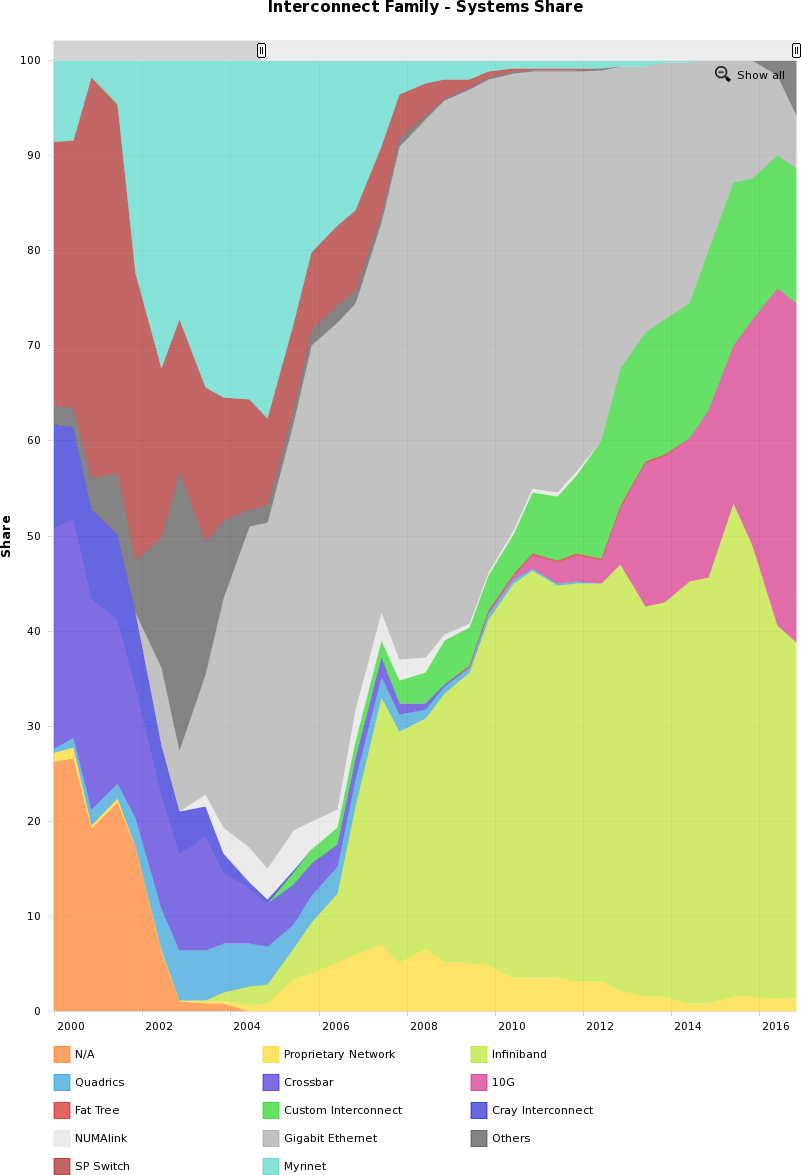
\includegraphics[width=\linewidth]{top500/interconnect/Interconnect_System}
\end{figure}
\end{minipage}
\begin{minipage}[bc]{0.4\linewidth}
\centering
\begin{figure}
\centering
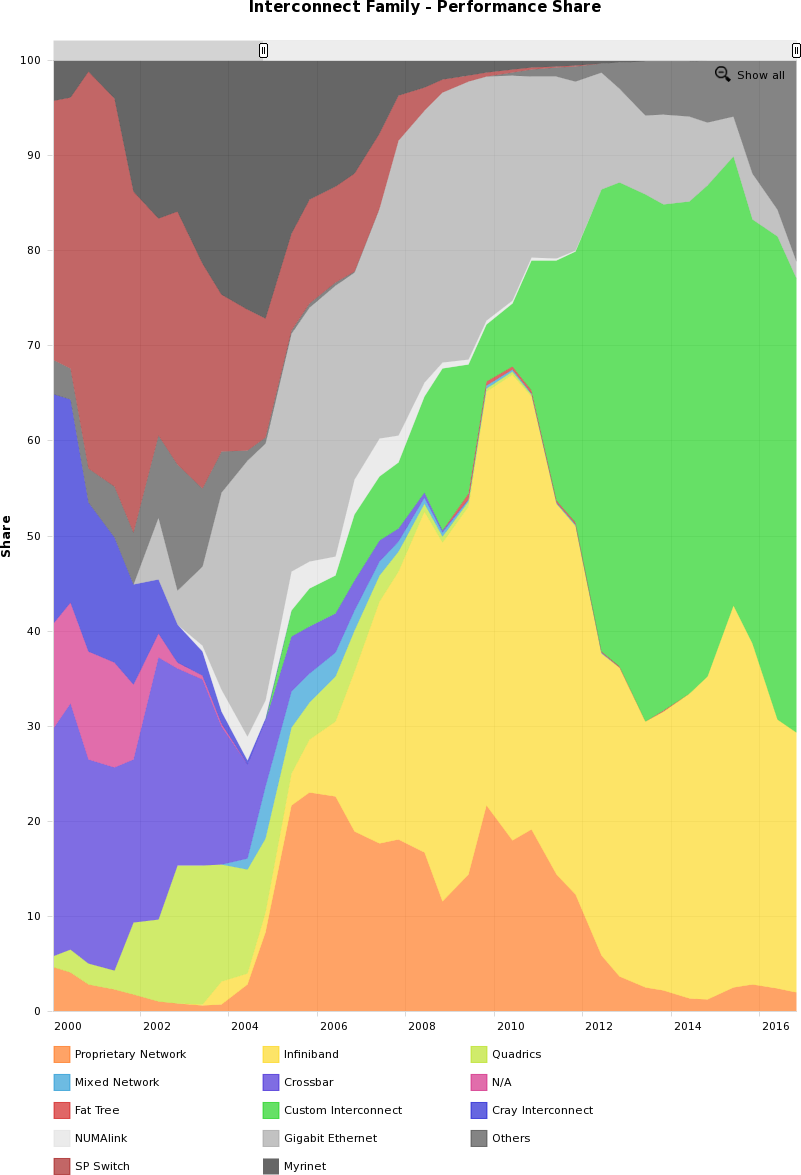
\includegraphics[width=\linewidth]{top500/interconnect/Interconnect_Performance}
\end{figure}
\end{minipage}

\smallskip
Comparison of the evolution w.r.t system and performance share.
\end{frame}

%----------------------------------------
\begin{frame}
  \frametitle{Efficiency: findings patterns}

\begin{figure}
\centering
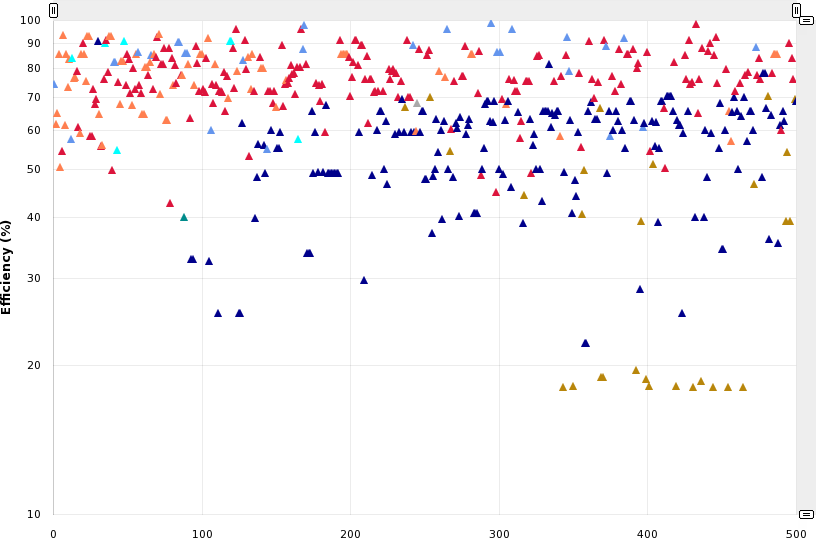
\includegraphics[width=0.7\linewidth]{top500/efficiency/Top500EfficiencyInterconnect}
\caption{Top500: Efficiency vs Interconnect}
\end{figure}

\end{frame}

%----------------------------------------
\begin{frame}
  \frametitle{Power efficiency: finding patterns}

\begin{figure}
\centering
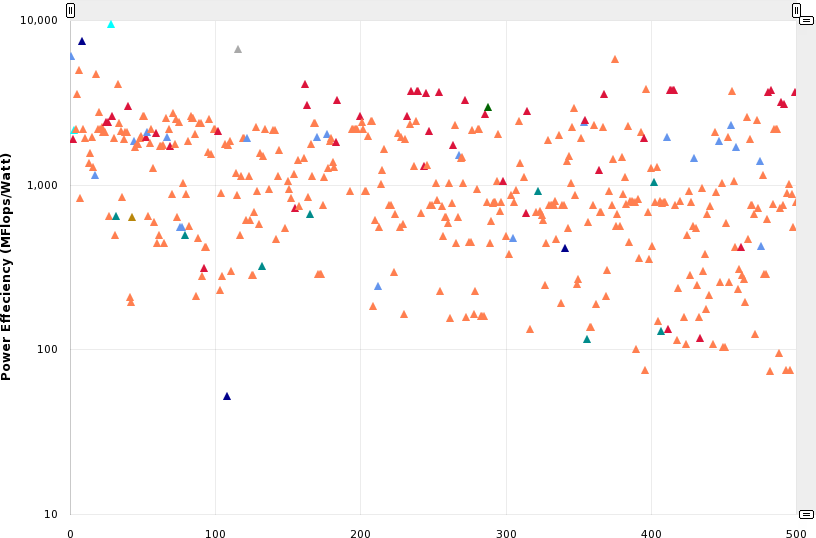
\includegraphics[width=0.7\linewidth]{top500/power/Top500PowerEfficiencyAccelerator}
\caption{Top500: Power Efficiency vs Accelerator}
\end{figure}

Cost: top supercomputers' energy cost per year is $\sim$ million dollar.
If energy consumption scales linearly: 1/10 nuclear power plant per Exascale supercomputer.

\end{frame}

%----------------------------------------
\begin{frame}
  \frametitle{Performance considerations}

\begin{figure}
\centering
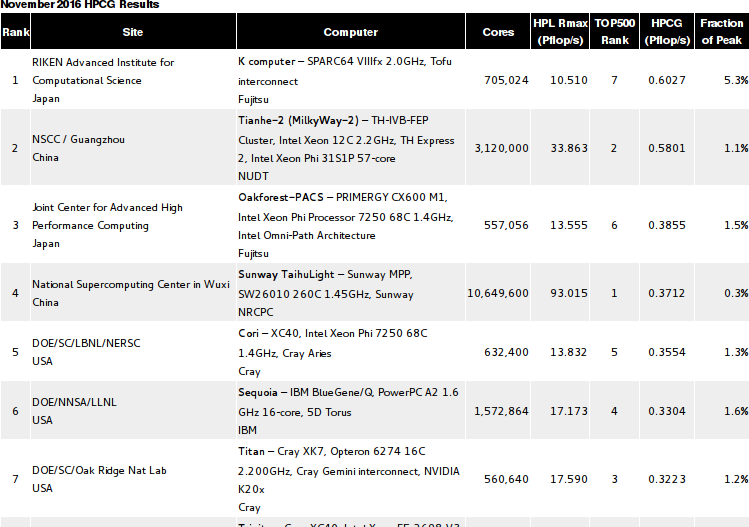
\includegraphics[width=0.7\linewidth]{hpcg/HPCGTop7}
\caption{High Performance Conjugate Gradients (HPCG) Benchmark project}
\end{figure}

Complement to LINPACK: dense vs sparse matrix computations.

\end{frame}

%------------------------------------------------------------------------------
\section{Conclusion}

\begin{frame}
  \frametitle{Conclusion}

\begin{itemize}
\item Supercomputing is crucial for Computer Science and Engineering to address new problems.
\item Development of computational power is enabling but poses challenges.
\item Adapting algorithms to compute on concurrent and parallel systems is non-trivial: application-dependent, low-level.
\item Various hardware architecture, programming models, languages available.
\item Communication is the key element in scalability.
\end{itemize}
\end{frame}

\end{document}

